\section{Method}

We did a series of experiments to achieve "cashier-free supermarket".
Include make scene to simulate a real supermarket and use multi cameras to cover whole scene to get  images which used to identity items types and number on shelves.

\subsection{Multi cameras and Build scene}
We build the Multi cameras scene is based on field of view(FOV), the horizontal field of view(H-FOV) and vertical field of view(V-FOV)\cite{Ball88} determined the sharpness and size of the pictures what we get.

\begin{figure}[htbp]
\centerline{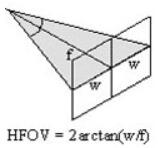
\includegraphics[width=2.5cm,scale=0.4]{HFOV.jpg} 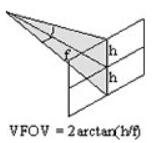
\includegraphics[width=2.5cm,scale=0.4]{VFOV.jpg}}
\caption{H-FOV and V-FOV .}
\label{fig}
\end{figure}

Fixed focal length lens, it can get the angel field of view(AFOV), and we can get different size of FOV through adjusting the focal length of the lens through different working distances.

\centerline{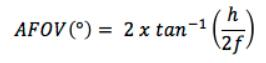
\includegraphics[width=5cm,scale=0.9]{AFOV-MA.jpg}}
\begin{figure}[htbp]
\centerline{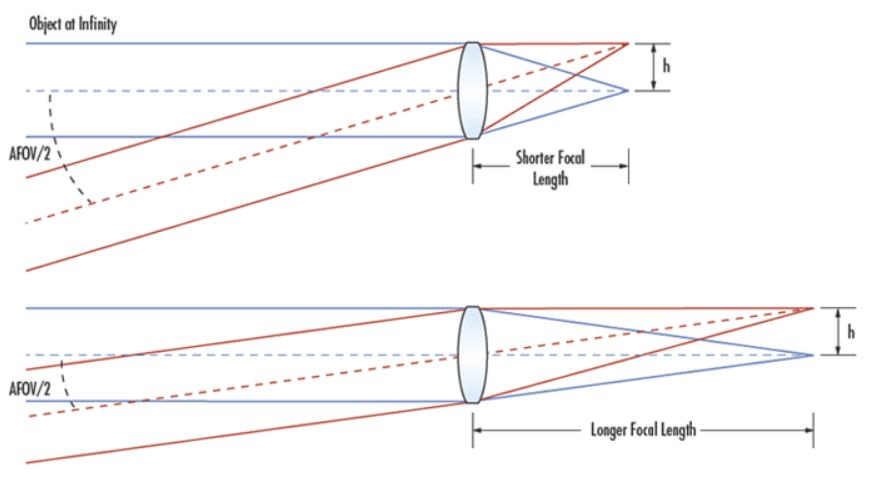
\includegraphics[width=9cm,scale=0.9]{AFOV.jpg}}
\caption{The field of view of lens is related to focal length, f is the focal length, h is the horizontal dimension of the sensor.}
\label{fig}
\end{figure}

We can follow the specifications of the scene (shelves size, the length and width of walking, and layout of the whole scene) to adjust FOV.

\subsection{Cameras selected}

The terms "dots per inch" (DPI) and "pixels per inch"(PPI) are used interchangeably by many. A 200 dpi print means that for each inch of that printed material, it takes about 200 dots to make the picture. A pixel is like a square dot without gaps. Both of them can describe the quality of a picture, and some cameras save digital images in arbitrary values as 72 dpi. We can calculate the DPI or PPI for what we need page size in Fig.3.
\begin{figure}[htbp]
\centerline{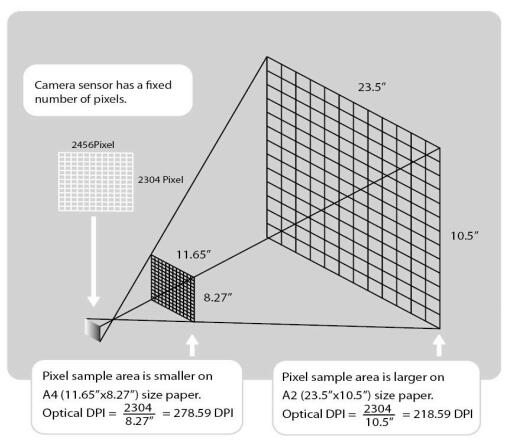
\includegraphics[width=8cm,scale=0.9]{DPIPPI.jpg}}
\caption{Page Size and Optical Resolution}
\label{fig}
\end{figure}

FLEXIDOME IP panoramic 7000 MP, which has 12MP / 30 fps sensor for fine details with smooth motion and Intelligent Video Analysis on full panoramic overview. Panoramic surveillance offers full 180° or 360° coverage of the designated area. The 360° version of the camera, when mounted
centrally on a ceiling, gives complete wall-to-wall coverage. The 180° version has a higher effective resolution and is ideal for wall mounting or for ceiling
mounting in corridors.

When mounted at a height of 3.5 m (11.48 ft) the 360° version of the camera has the following coverage radius for the four levels in Fig.4.
\begin{figure}[htbp]
\centerline{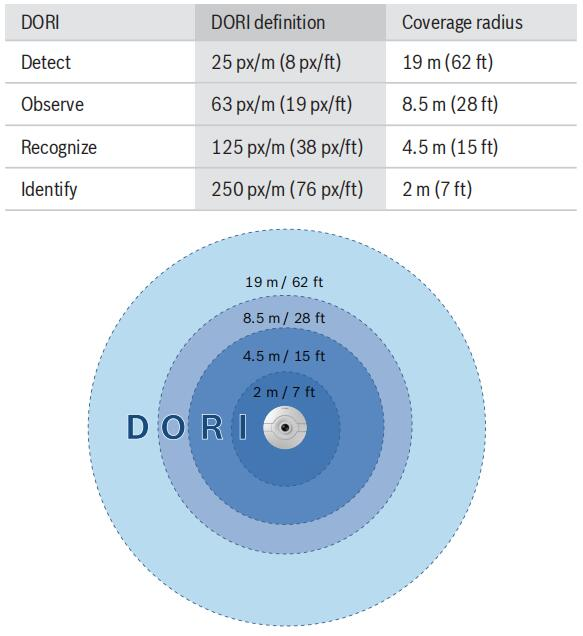
\includegraphics[width=7cm,scale=0.8]{camera360.jpg}}
\caption{Page Size and Optical Resolution}
\label{fig}
\end{figure}

When mounted at a height of 3.5 m (11.48 ft) the 180° version of the camera has the following coverage radius for the four levels in Fig.5.
\begin{figure}[htbp]
\centerline{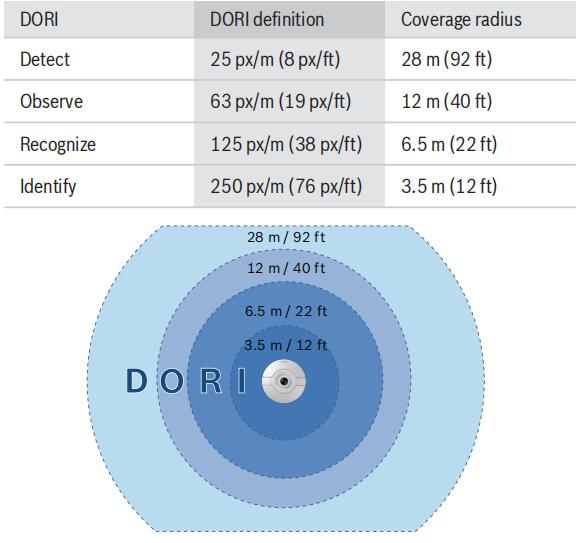
\includegraphics[width=7cm,scale=0.8]{camera180.jpg}}
\caption{Page Size and Optical Resolution}
\label{fig}
\end{figure}

\subsection{Identity items}

\subsection{Item Recognition}

\subsection{sensor fusion}
